\documentclass{template}

% --- PACKAGES ---
% \usepackage[margin=1in, headheight=14pt, top=1.2in]{geometry}
% \usepackage{amsmath,amssymb}
% \usepackage{graphicx}
% \usepackage{enumitem}
% \usepackage{hyperref}
% \usepackage{fancyhdr}
% \usepackage{float}
\usepackage{xcolor}
\usepackage{mdframed}
\usepackage{etoolbox}
\usepackage{pdfpages}
\usepackage{cancel}

\graphicspath{{attachments/}}

% --- TOGGLE FOR ANSWERS ---
% Set to \toggletrue{showanswers} to display answers.
% Set to \togglefalse{showanswers} to hide answers.
\newtoggle{showanswers}
\toggletrue{showanswers}

% --- CUSTOM SOLUTION ENVIRONMENT ---
\newmdenv[
  backgroundcolor=white,
  linecolor=blue!60!black,
  linewidth=1.5pt,
  topline=false,
  rightline=false,
  bottomline=false,
  leftmargin=2pt,
  innerleftmargin=10pt,
  innertopmargin=6pt,
  innerbottommargin=6pt,
  skipabove=8pt,
  skipbelow=8pt
]{solutionbox}

\newcommand{\solution}[1]{%
\iftoggle{showanswers}{%
\begin{solutionbox}
        #1
\end{solutionbox}%
  }{}%
}

% \usepackage[]{opensans} % Loads Open Sans font family
% \newcommand{\solution}[1]{%
%   \iftoggle{showanswers}{%
%     \begin{solutionbox}
%         \fontsize{10}{12}\opensans #1
%     \end{solutionbox}%
%   }{}%
% }

\addbibresource{hw3_biber.bib}


% --- HEADER & FOOTER CONFIGURATION ---
\pagestyle{fancy}
\fancyhf{}
\lhead{\textbf{EEPS 5534: Interior of the Earth}}
\rhead{\textbf{Problem Set 3}}
\cfoot{\thepage}


\title{\textbf{Problem Set 3}}
\author{Nathalie Redick}
\date{Due: Nov. 11, 2026}

\begin{document}

\maketitle
\thispagestyle{fancy}

\begin{enumerate}[label=\textbf{\arabic*.}]

% ------------------------------------------------------------
% QUESTION 1
% ------------------------------------------------------------
\item It is likely that other terrestrial planets have a mantle composition similar to Earth's. Estimate the depths of the olivine mineral phase transitions for Mars.

First, calculate and plot the pressure as a function of depth in the Martian mantle using equation 2.73 from \textcite{turcotteGeodynamics2014} (given below).

Then, use the phase diagram given below to estimate the pressures of the olivine-wadsleyite, wadsleyite-ringwoodite, and ringwoodite-bridgmanite+magnesiowustite phase transition. Note that the phase diagram is from an old publication, so "mod Sp" = wadsleyite, "Sp" = ringwoodite, and "Pv" = bridgmanite.

Assume that the temperature of the Martian mantle at the depths of the phase change is similar to the Earth's transition zone, that the Mg\# is 80 (instead of 90, as for the Earth), the radius of Mars' core is 1700 km, and the average density of Mars' mantle and core are \qty{3500}{\kg\per\m\cubed} and \qty{6500}{\kg\per\m\cubed}.

Does Mars' mantle have the same transitions as found in Earth's transition zone? If so, at what depth would the discontinuities be found, and, if they are not sharp, give the depth range of the discontinuity.\\

Equation 2.73 from \textcite{turcotteGeodynamics2014}:

% * reference Problem 2.18 in T & S 2014
\begin{align}
p(r) &= \frac{4}{3}\pi\rho_m G b^3(\rho_c - \rho_m)\left(\frac{1}{r} - \frac{1}{a}\right)
      + \frac{2}{3}\pi G \rho_m^2 (a^2 - r^2)
      && b \leq r \leq a \nonumber \\
     &= \frac{2}{3}\pi G \rho_c^2 (b^2 - r^2)
      + \frac{2}{3}\pi G \rho_m^2 (a^2 - b^2) \nonumber
      + \frac{4}{3}\pi\rho_m G b^3(\rho_c - \rho_m)\left(\frac{1}{b} - \frac{1}{a}\right)
      && 0 \leq r \leq b
      \tag{2.73} % ! it's actually eqn 2.73
\end{align}

% \begin{figure}[H]
%     \centering
%     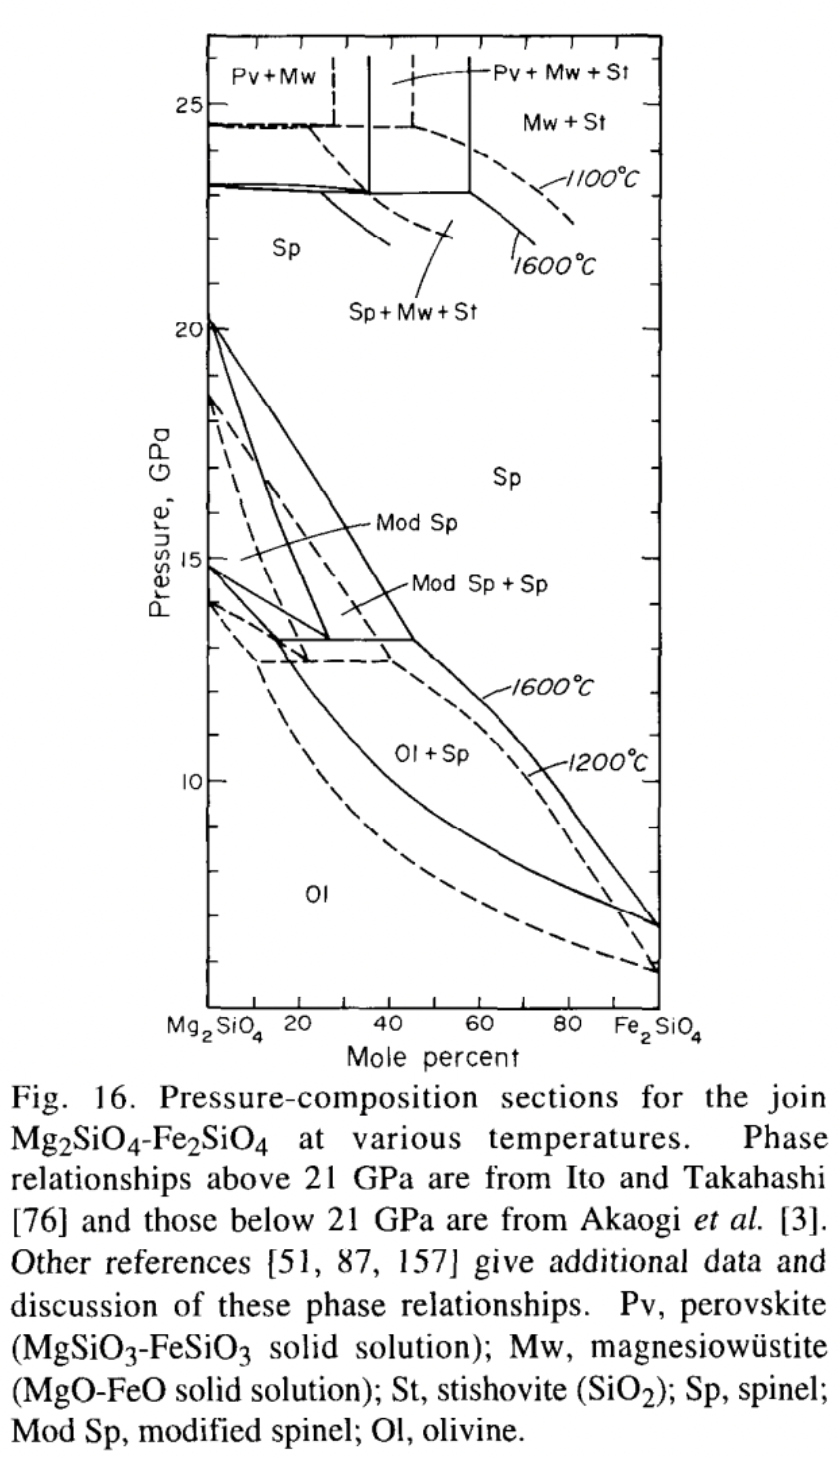
\includegraphics[width=0.5\textwidth]{fig-16}
%     % \caption{CAPTION}
%     \label{fig:fig-16}
% \end{figure}

\solution{

    \begin{figure}[H]
        \centering
        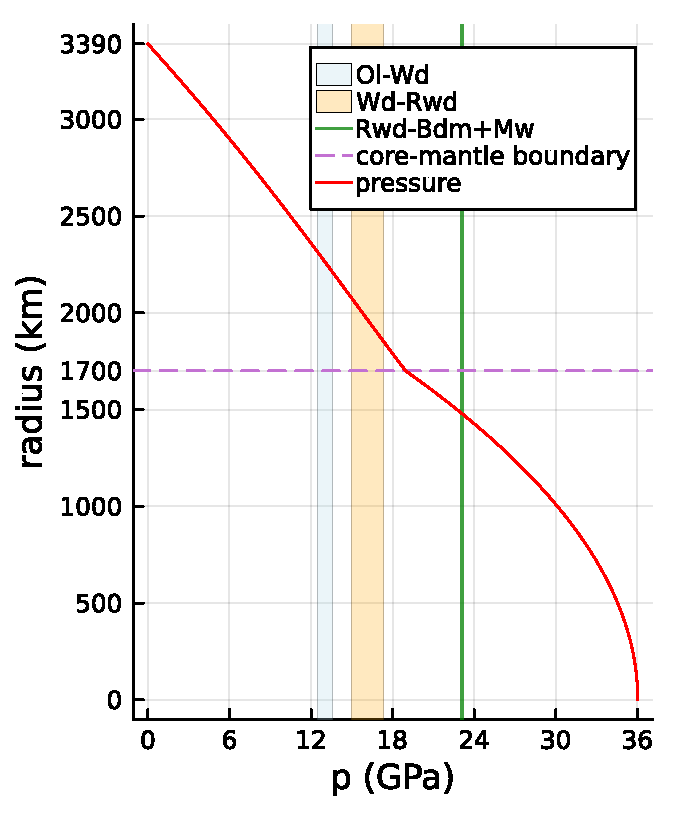
\includegraphics[height=0.45\textheight]{q1-pressure_v_depth}
        \caption{Pressure in GPa (red) vs. radius (km) of the Martian mantle, assuming a two-layer (core and upper mantle) structure. Estimated pressure ranges for olivine phase transitions shown, based on the provided figure (assuming the temperature of the Martian mantle at the depths of the phase change is similar to Earth's transition zone at about \qty{1600}{\celsius}). Julia notebook codes used to create the plot are attached at the end.}
        \label{fig:q1-pressure_v_depth}
    \end{figure}

    Assuming a Mg\# 80 for Mars, the pressures of the phase transitions lie along the vertical line at 20 mol\% between \ce{Mg2SiO4}--\ce{Fe2SiO4}. Even with the shift in the Mg\#, the Mars' mantle experiences only the Ol-Wd and Wd-Rwd phase transitions, because the pressure condition required for the Rwd-Bdm+Mw transition would only occur in the core. The pressure ranges of the transitions can be determined approximately from the provided figure (see annotations on Figure~\ref{fig:q1-annot_fig}), and the depth ranges can be estimated* from the pressure vs. radius plot (Figure~\ref{fig:q1-pressure_v_depth}):

    \begin{table}[H]
    \centering
    \begin{tabular}{lll}
    \hline
    Phase Transition & Pressure (GPa) & Radius ($\pm25$ km) \\ \hline
    Ol-Wd            & 12.5--13.6     & 2325--2200 \\
    Wd-Rwd           & 15--17.3       & 2075--1850 \\
    % Rwd-Bdm+Mw       & 23.1           & 1475       \\ \hline
    \end{tabular}
    \end{table}

    \begin{figure}[H]
        \centering
        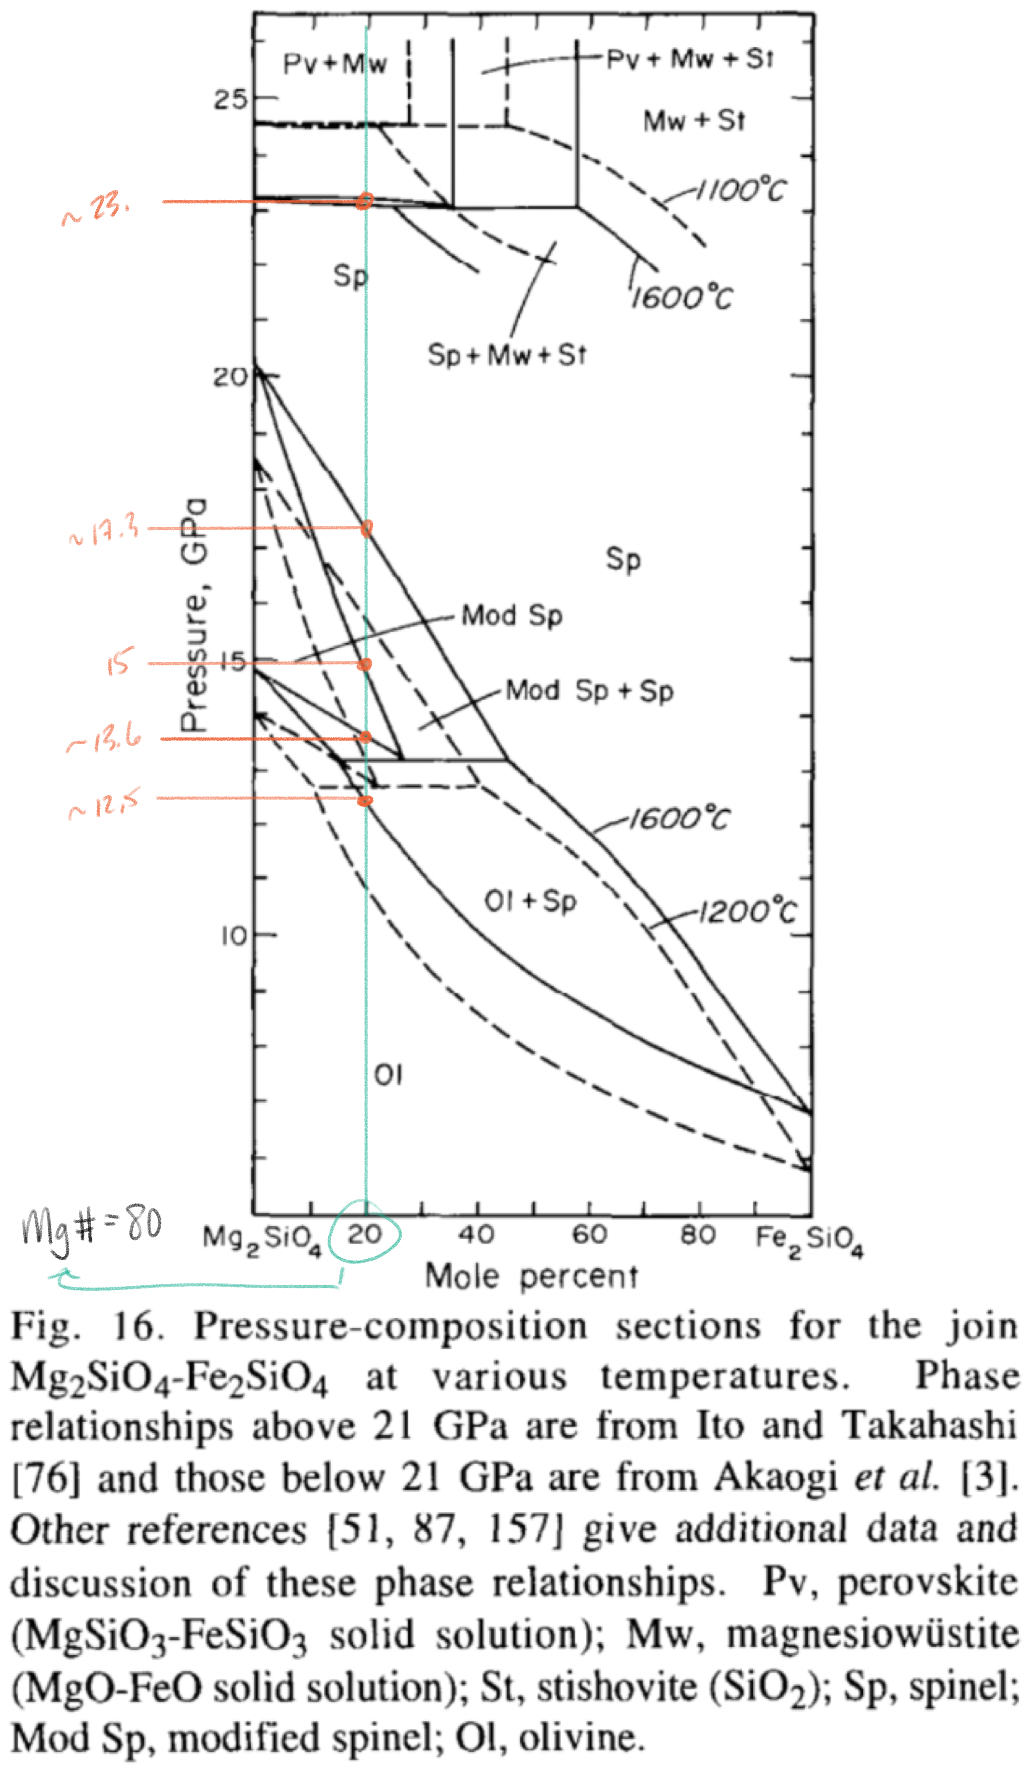
\includegraphics[height=0.75\textheight]{q1-annot_fig}
        \captionof{figure}{Annotated phase relationships, 20 mol\% line (green) at Mg\# = 80.}
        \label{fig:q1-annot_fig}
    \end{figure}

    *estimated by blowing up the height of the plot and setting the y-ticks every 25 km.
}

\newpage
\item Consider the effects of composition and temperature on the elevation of continental cratons. Assume for simplicity that the continental crust and mantle lithosphere beneath it are originally 35 km and 65 km thick, respectively. Assume that the temperature at the base of the crust remains a constant \qty{500}{\celsius}, that the temperature of the asthenosphere immediately below the lithosphere is \qty{1400}{\celsius}, that the average density of the upper mantle is \qty{3300}{\kg\per\m\cubed}, and that the lithosphere has a linear conductive thermal gradient.

\begin{enumerate}[label=\Alph*)]

    \item Use the principle of isostasy (the mass in a column remains constant down to the depth of compensation---generally assumed to be the asthenosphere) and the coefficient of thermal expansion ($\alpha\sim$ \qty{2.5e-5}{\celsius^{-1}}) to calculate the change in elevation of the craton that would occur if the thickness of the thermal lithosphere doubled through cooling over time. Note that you can make this calculation easy (but still correct) by assuming that all the mantle lithosphere is at the average mantle lithosphere temperature. So the lithosphere stays at the same average temperature and density, but doubles in thickness.

    \solution{
        \begin{figure}[H]
            \centering
            \begin{subfigure}[t]{0.49\textwidth}
                \centering
                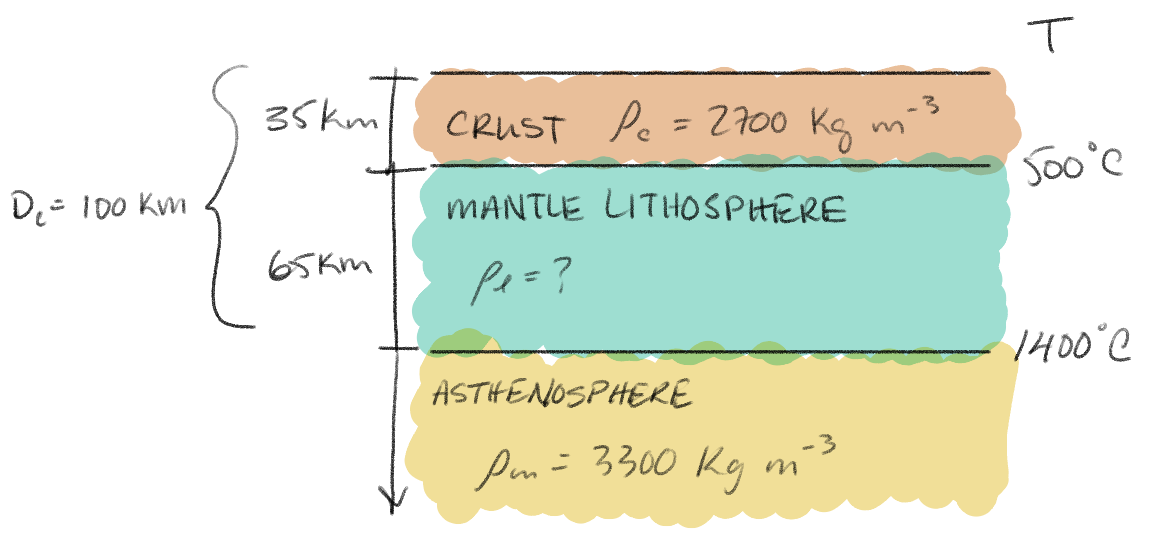
\includegraphics[width=\textwidth]{q2a-initial}
                % \caption{Initial state: 35 km crust ($\rho_c = 2700$ kg/m$^3$) over 65 km mantle lithosphere ($\rho_L \approx 3337$ kg/m$^3$), for a 100 km thermal lithosphere above asthenosphere ($\rho_a = 3300$ kg/m$^3$, 1400\,\textdegree C).}
                % \label{fig:q2a-initial}
            \end{subfigure}\hfill
            \begin{subfigure}[t]{0.49\textwidth}
                \centering
                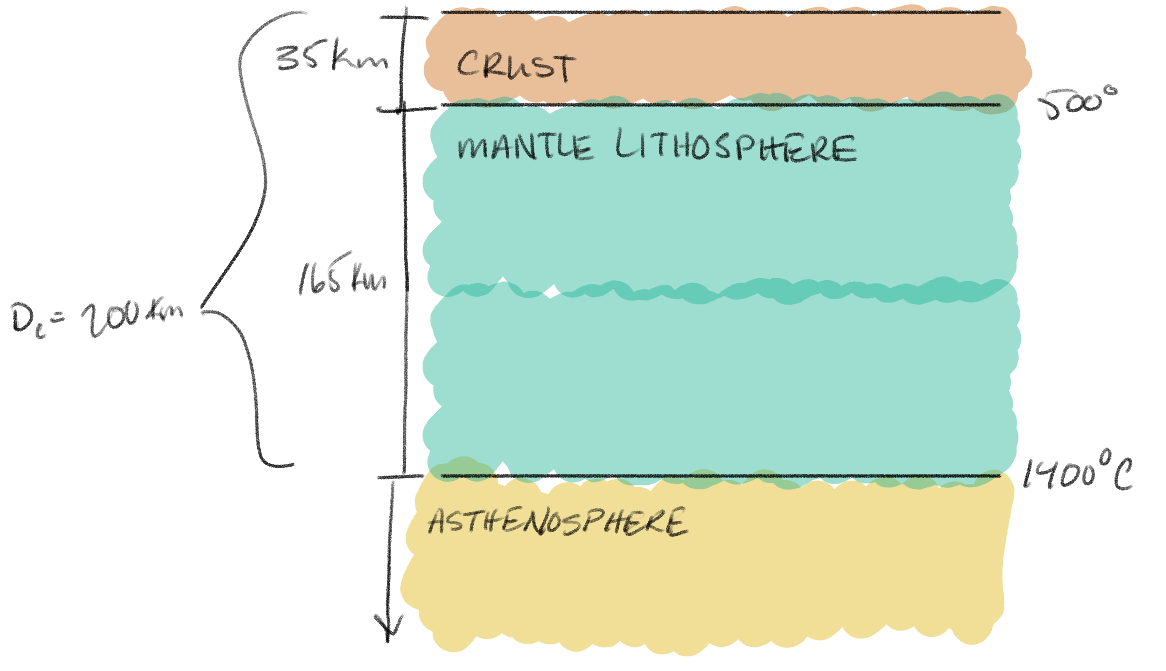
\includegraphics[width=\textwidth]{q2a-cooled}
                % \caption{After cooling: the thermal lithosphere is 200 km thick (same 35 km crust, 165 km mantle lithosphere at the same $\rho_L$). The surface has dropped $x \approx 1.1$ km to keep the mass above the compensation depth $D$ constant.}
                % \label{fig:q2a-cooled}
            \end{subfigure}
            \caption{Schematics showing a craton that experiences doubling of the thermal lithosphere thickness by cooling from 100 to 200 km. Initial state on the left, present (cooled) state on the right.}
        \end{figure}

        \begin{itemize}
            \item $D_{c[i,f]}$ = compensation depth (\textit{i} = initial, \textit{f} = final)
            \item $\rho_c$ = density of the crustal lithosphere
            \item $\rho_l$ = density of the mantle lithosphere
            \item $\rho_m$ = density of the asthenospheric mantle\\
        \end{itemize}

        Assuming that "thermal lithosphere" refers to the entire 100 km of the lithosphere, doubling the thickness of the lithosphere results in a 200 km thick lithosphere, where the additional 100 km is cooled and captured asthenospheric material, which becomes a part of the mantle lithosphere (crustal thickness remains 35 km). This mantle lithosphere material has the same composition as the asthenosphere, and has a linear conductive geothermal gradient, therefore the average temperature of the mantle lithosphere (both initially and after cooling) is:

        \begin{align*}
            T_{\text{avg}} &= \frac{500+1400}{2} = \qty{950}{\celsius}
        \end{align*}

        Assume that all the mantle lithosphere is at this average temperature.\\

        The density ($\rho_l$) of the mantle lithosphere is determined by thermal contraction during cooling relative to the given coefficient of thermal expansion, such that:
        \begin{align*}
            \rho_l &= \rho_m \cdot \alpha (1 - \Delta T)\\
            &= \qty{3300}{\kg\per\m\cubed} \cdot \qty{2.5e-5}{\celsius^{-1}} (1 - (\qty{950}{\celsius} - \qty{1400}{\celsius}))\\
            &\approx \qty{3337}{\kg\per\m\cubed}
        \end{align*}

        Using the isostatic principle, the change in the elevation ($x$) of the cooled craton can be determined by setting up a mass balance for the initial ($M_i$) and final ($M_f$) states of the system. Since we are working in a 2D system, $m = \rho \cdot A$, where $A$ is the area of the column; however, the width of the column is constant and arbitrary, such that $m = \rho \cdot h$, where $h$ is the height of the column.\\

        % Additionally, I use $\rho_c = \qty{2700}{\kg\per\m\cubed}$ \parencite[assuming an average granodioritic composition, using the value from Appendix B, Section B.5 of][]{turcotteGeodynamics2014} for the crustal lithosphere.\\

        Mass balance:

        \begin{align*}
            M_i &= M_f\\
            \rho_c h_c + \rho_l h_{l,i} + \rho_m (D_c - (h_c + h_{l,i})) &= \rho_c h_c + \rho_l h_{l,f} + \rho_m ((D_c + x) - (h_c + h_{l,f}))\\
            \cancel{\rho_c h_c} + \rho_l h_{l,i} - \rho_l h_{l,f} + \rho_m (D_c - (h_c + h_{l,i})) &= \cancel{\rho_c h_c} + \rho_m ((D_c + x) - (h_c + h_{l,f}))\\
            \frac{\rho_l h_{l,i} - \rho_l h_{l,f} + \rho_m (D_c - (h_c + h_{l,i}))}{\rho_m} &= (D_c + x) - (h_c + h_{l,f})\\
            x &= \frac{\rho_l h_{l,i} - \rho_l h_{l,f} + \rho_m (D_c - (h_c + h_{l,i}))}{\rho_m}\\&\quad + h_c + h_{l,f} - D_c \\
            % x &= \frac{\rho_l h_{l,i}}{\rho_m} - \frac{\rho_l h_{l,f}}{\rho_m} + \cancel{D_c} - \bcancel{h_c} - h_{l,i} + \bcancel{h_c} + h_{l,f} - \cancel{D_c} \\
            &= \frac{\rho_l h_{l,i}}{\rho_m} - \frac{\rho_l h_{l,f}}{\rho_m} + h_{l,f} - h_{l,i} \\
            &= (h_{l,f} - h_{l,i})\,\frac{\rho_m - \rho_l}{\rho_m} \\
            &= (165-65)\unit{\km} \left( \frac{3300 - 3337}{3300} \unit{\kg\per\m\cubed}\right)\\
            &\approx \boxed{\qty{-1.12}{km}}
        \end{align*}

        Doubling the thickness of the lithosphere via cooling results in \textbf{subsidence} of $\sim \qty{1.12}{km}$.
    }

    \newpage
    \item Now calculate the change in elevation expected if the original 65 km thick lithosphere goes from "normal" upper mantle to upper mantle depleted in iron. Assume that the derivative of density with respect to Mg\# is \qty{-12}{\kg\per\m\cubed} Mg\#\textsuperscript{-1} [Akimoto, 1972], where Mg\# is 100*Mg/(Mg+Fe) in the olivine forsterite-fayalite solid solution. Assume that the depletion changes the Mg number from 89 to 94, and that the lithosphere remains 65 km thick.

    \solution{
        \begin{itemize}
            \item $\frac{\partial \rho}{\partial \mathrm{Mg\#}} = \qty{-12}{\kg\per\m\cubed}\,\mathrm{Mg\#}^{-1}$
            \item $\mathrm{Mg\#} = \frac{100 \cdot \ce{Mg}}{\ce{Mg}+\ce{Fe}}$
        \end{itemize}

        Setting up the same mass balance as before:

        \begin{align*}
            M_{[89]} &= M_{[94]}\\
        \end{align*}

        \begin{align*}
            \frac{\partial \rho}{\partial \mathrm{Mg\#}} &= \qty{-12}{\kg\per\m\cubed} \,\mathrm{Mg\#}^{-1} \\
            \Delta \mathrm{Mg\#} &= 94 - 89 = 5 \\
            \Delta\rho &= \left(\frac{\partial \rho}{\partial \mathrm{Mg\#}}\right)\left(\Delta \mathrm{Mg\#}\right) \\
            &= (-12)(5) \\
            &= \qty{-60}{\kg\per\m\cubed} \\
            \rho_{[94]} &= \rho_{[89]} + \Delta\rho \\
            &= 3300 - 60 \\
            &= \qty{3240}{\kg\per\m\cubed}
        \end{align*}

        \begin{align*}
            \cancel{\rho_c h_c} + \rho_{[89]}\,h_l + \rho_m\bigl(D_c - (h_c + h_l)\bigr)
            &= \cancel{\rho_c h_c} + \rho_{[94]}\,h_l + \rho_m\bigl(D_c + x - (h_c + h_l)\bigr) \\
            \rho_{[89]}\,h_l - \rho_{[94]}\,h_l + \cancel{\rho_m}\bigl(D_c - (h_c + h_l)\bigr)
            &= \cancel{\rho_m}\bigl(D_c + x - (h_c + h_l)\bigr) \quad (\div\,\rho_m) \\
            \frac{\rho_{[89]}\,h_l}{\rho_m} - \frac{\rho_{[94]}\,h_l}{\rho_m}
            + \cancel{D_c} - \bcancel{h_c} - \xcancel{h_l}
            &= \cancel{D_c} + x - \bcancel{h_c} - \xcancel{h_l} \\
            \frac{\rho_{[89]}\,h_l}{\rho_m} - \frac{\rho_{[94]}\,h_l}{\rho_m} &= x \\
            x &= \frac{(3300)(65)}{3300} - \frac{(3240)(65)}{3300} \\
            &\approx \boxed{+\qty{1.18}{km}}
        \end{align*}

        The depletion of the lithospheric mantle results in an \textbf{uplift} of $\sim \qty{1.18}{km}$.

    }

    \item Now calculate the change in elevation expected if the original 65 km thick undepleted lithosphere is thickened due to cooling and depleted due to iron extraction at the same time. What conclusions can you draw about the effect of different processes on continental lithosphere?

    \solution{
        % todo q2c
    }
\end{enumerate}

\newpage
\item The amount of water in the MORB (mid-ocean ridge basalt) source is estimated as 0.01 wt \% (100 ppm) on average.

\begin{enumerate}[label=\Alph*)]

    \item If the entire mantle contained this percentage of water, how much water would this be? How does this compare to the total amount of water in the oceans?

    \solution{

        Using the mass of Earth's mantle as \qty{4004e21}{\kg}, given by Table 8.1 of \textcite{fowlerSolidEarthIntroduction2012}, the amount of water can be calculated as:

        \begin{align*}
            \qty{4004e21}{\kg} \cdot \frac{\qty{0.01}{\percent}}{100} &\approx \boxed{\qty{4.004e20}{\kg}}
        \end{align*}

        Assuming the Earth's oceans have an approximate mass of \qty{1.4e21}{\kg} \parencite{Vallis2012}, this estimate suggests there is significantly more water in the mantle than in Earth's oceans (amount of water in the mantle is $\sim0.29$ times greater).
    }

    \item The amount of water inferred for plume mantle source rocks is considerably larger, on the order of 0.05 wt \%. Redo the calculation in A) assuming that the entire mantle contains this amount of water on average.

    \solution{
        \begin{align*}
            \qty{4004e21}{\kg} \cdot \frac{\qty{0.05}{\percent}}{100} &\approx \boxed{\qty{2.002e21}{\kg}}
        \end{align*}

        This increases the estimate to $\sim1.4$ times greater than the mass of water in Earth's oceans.
    }

    \item “Wet” models of the earth’s interior usually propose significant amounts of water in the transition zone, between the 410 km discontinuity and the 660 km discontinuity. The storage capacity of water in transition zone olivine (wadsleyite and ringwoodite) is thought to be about 1 wt \%. Make a calculation to estimate the amount of water in the transition zone if it is saturated. Express your answer in units of “oceans”.

    \solution{

        Volume of the transition zone (estimated using a spherical shell, with radii measured from Earth's center:

        \begin{align*}
            V &= \frac{4}{3}\pi \left[ (6371 - 410)^3 - (6371 - 660)^3 \right] \qty{}{\km\cubed}\\
            &= \frac{4}{3}\pi \left[ 5961^3 - 5711^3 \right] \qty{}{\km\cubed}\\
            &\approx \qty{1.07e11}{\km\cubed}
        \end{align*}

        Assuming a pyrolite model, wadsleyite + ringwoodite make up $\sim 60$ vol.\% of the transition zone \parencite{ChangetalComparativeCompressibility2015}:

        \begin{align*}
            V_{\text{ol}} &= 0.6 \times \qty{1.07e11}{\km\cubed}\\
            &\approx \qty{6.42e10}{\km\cubed} = \qty{6.42e19}{\m\cubed}
        \end{align*}

        Convert to mass, assuming an average $\rho \approx \qty{4000}{\kg\per\m\cubed}$ for the olivine phases in the transition zone \parencite{ALEXSTREKEISENOlivine}:

        \begin{align*}
            m &= \rho V \\
            &= \left(\qty{4000}{\kg\per\m\cubed}\right)\left(\qty{6.42e19}{\m\cubed}\right)\\
            &\approx \qty{2.57e23}{\kg}
        \end{align*}

        Mass of water at saturation (1 wt\%):

        \begin{align*}
            \qty{2.57e23}{\kg} \cdot \frac{\qty{1}{\percent}}{100} &\approx \qty{2.57e21}{\kg}\\
            \implies \frac{\qty{2.57e21}{\kg}}{\qty{1.4e21}{\kg\per ocean}} &\boxed{\approx \qty{1.8}{oceans}}
        \end{align*}

    }
\end{enumerate}

\newpage
\item The eruption rate of volcanoes in Iceland greatly increased about 11 kyr years ago. This has been attributed to increased decompression melting in the mantle due to the reduction of pressure resulting from deglaciation, during which a 1.5 km thick ice sheet disappeared around 12 kyr ago.

\begin{enumerate}[label=\Alph*)]

    \item Calculate the decrease in pressure in the mantle due to the removal of the ice sheet. Ignore any geometric effects caused by the finite geographical size of the ice sheet.

    \solution{

        Ignoring any geometric effects implies that the change in pressure is not laterally heterogeneous. The pressure in the mantle is the sum of the pressure applied by the overriding ice sheet, the lithosphere, and the overlying air column. Assuming that the lithosphere and air column are unchanged, the decrease in pressure can be calculated as follows, taking the density of ice ($\rho_{\text{ice}}$) as \qty{917}{\kg\per\m\cubed}:

        \begin{align*}
            \Delta P &= \rho_{\text{ice}} g h\\
            &= \qty{917}{\kg\per\m\cubed} \cdot \qty{9.81}{\m\per\s\squared} \cdot \qty{1.5e3}{\m}\\
            &\approx \boxed{\qty{13.5}{\MPa}}
        \end{align*}
    }

    \item Decompression melting normally occurs through mantle upwelling beneath mid-ocean ridges or plumes. Compare the amount of decompression from the ice sheet with mantle upwelling by calculating the distance that mantle material would have to rise in order to have the same amount of pressure reduction.

    \solution{

        Assuming again no lateral heterogeneity and an upper mantle density of $\rho_{m}=\qty{3300}{\kg\per\m\cubed}$, the amount of mantle upwelling required to achieve a pressure reduction of \qty{13.5}{\MPa} is:

        \begin{align*}
            h &= \frac{\Delta P}{\rho_{m}g}\\
            &= \frac{\qty{1.35e7}{\Pa}}{\qty{3300}{\kg\per\m\cubed}\cdot\qty{9.81}{\m\per\s\squared}}\\
            &= \boxed{\qty{417}{\m}}
        \end{align*}

    }

    \item This model implies that melt is transported from the depths of mantle melting to the surface between the time of deglaciation and the time of massive volcanism. Give an order-of-magnitude estimate of the average vertical melt transport speed indicated by this scenario.

    \solution{

        Assuming a mantle melting depth of $\sim\qty{100}{\km}$ beneath Iceland, the average vertical melt transport speed can be calculated as:

        \begin{align*}
            v &= \frac{d}{t}\\
            &= \frac{\qty{100}{\km}}{\qty{12}{kyr} - \qty{11}{kyr}}\\
            &= \frac{\qty{100}{\km}}{\qty{1000}{ yr}}\\
            &= \qty{0.1}{\km\per yr} = \boxed{\qty{100}{\m\per yr} }%\approx \boxed{\qty{3e-6}{\m\per\s}}
        \end{align*}

        This is fast, but consistent with constraints on melt speed in the upper mantle that indicate melt transport speeds in the range of 1--100\unit{\m\per yr} \parencite{KatzPhysicsofMeltExtraction2022}.

    }
\end{enumerate}

\newpage
\item Make a back-of-the envelope calculation about uplift in the Canadian shield from deglaciation. Make the assumption that the deglaciation occurred 12,000 years ago, that the original depression of the land during the glacial maximum was 1 km, that the dominant wavelength of the Laurentide ice sheet was 5000 km, and that the mantle viscosity is \qty{2e21}{\Pa\s} (an average of estimated upper and lower mantle viscosities).

\begin{enumerate}[label=\Alph*)]

    \item How much uplift remains to occur in the future?

    \solution{

        $$ E = E_0\cdot e^{-t/\tau};\quad \tau = \frac{4 \pi \eta}{\rho g \lambda} $$

        \begin{align*}
            \tau &= \frac{4 \pi \cdot \qty{2e21}{\Pa\s}}{\qty{3300}{\kg\per\m\cubed} \cdot \qty{9.81}{\m\per\s\squared} \cdot \qty{5e6}{\m}} \\
            &\approx \qty{1.55e11}{\s} \approx \qty{4.9e3}{yr}\\
            E &= \qty{1}{\km}\cdot e^{-(\qty{12000}{\km})/(\qty{4.9e3}{yr})}\\
            &\approx \boxed{\qty{87.3}{\m}}
        \end{align*}

        About \qty{87}{\m} of uplift remains to occur.

    }

    \item What is the current uplift rate in mm/yr? You can calculate this either by taking the derivative, or by a finite difference method (calculate two time points and subtract)

    \solution{
        Using the derivative of the relaxation law:

        \begin{align*}
            \frac{dE}{dt} = -\frac{E_0}{\tau} e^{-t/\tau} = -\frac{E}{\tau}
        \end{align*}

        The present uplift rate is:

        \begin{align*}
            \left|\frac{dE}{dt}\right| &= \frac{\qty{87}{\m}}{\qty{4.9e3}{ yr}}\\
            &\approx \boxed{\qty{1.8e-2}{\m\per yr}} \approx \qty{18}{\mm\per yr}
        \end{align*}
    }

    \item Repeat the calculations from A) and B) with a viscosity of \qty{4e20}{\Pa\s}, appropriate for the upper mantle. How does the uplift depend on mantle viscosity?

    \solution{
        \begin{align*}
            \tau &= \frac{4\pi \cdot \qty{4e20}{\Pa\s}}{\qty{3300}{\kg\per\m\cubed} \cdot \qty{9.81}{\m\per\s\squared} \cdot \qty{5e6}{\m}}\\
                &\approx \qty{3.11e10}{\s} \approx \qty{984}{yr}\\
            E &= \qty{1}{\km} \cdot \exp\!\left(-\frac{\qty{12000}{yr}}{\qty{984}{yr}}\right)\\
            &\approx \boxed{\qty{5}{\mm}}
        \end{align*}

        The new uplift rate is:

        \begin{align*}
            \left|\frac{dE}{dt}\right| &= \frac{E}{\tau} = \frac{\qty{5e-3}{\m}}{\qty{984}{ yr}}\\
            &\approx \qty{5e-6}{\m\per yr} = \boxed{\qty{5}{\mm\per yr}}
        \end{align*}

        As viscosity decreases, the characteristic time decreases, therefore the rebound occurs more quickly, so less uplift remains to occur at the present day.
    }
\end{enumerate}

\end{enumerate}

% \section*{Acknowledgments}
% Conversion of questions from Word into LaTeX provided by Claude (October 2026 version). Plots produced in Python, with some formatting assistance from Google Gemini (v. Oct. 2026).

\singlespacing
\printbibliography[title={References}]

% todo add pdf of jupyter notebook

% \newpage

\end{document}